% Provenance (never printed): see sources/outline_sources.md (Year 1: insolation with
% latitude and season, the radiative surplus and deficit, meridional heat transport by
% the atmosphere and the ocean, latent heat). Exercise and problem values in the Book 3
% scratch calculator calc/ch27.py; figures from figdata/bachelor-1/insolation.py (Kepler
% orbit of _solar.py) and energy_balance.py (NCEP-NCAR Reanalysis 1, long-term means
% 1991-2020, datasets bachelor-1-ncep-*).
% Physics owns the inverse-square law, the black body and the Stefan-Boltzmann law, the
% seasons and latent heat (recalled). Book 2 (g10) gave the quarter of the solar constant,
% the global budget diagram and its closure, latent and sensible heat in words, the
% annual-mean insolation curve and the poleward transport in words: re-founded here with
% derivations and data. Ch. 1 gave the instantaneous insolation, the declination and the
% rising and setting of the Sun.
\chapter{Radiation and Heat Transport}\label{ch:b1:radiation-heat-transport}

From a million miles away, the sunlit face of the Earth is a disc of blue sea,
brown land and white cloud. The sunlight falls most directly on the middle of
the disc, near the tropics, and grazes its edges; the tropics absorb far more
energy than the polar regions. Yet the tropics do not grow hotter year after
year, nor the poles colder. Winds and ocean currents carry the excess towards
the poles, several petawatts of it. This chapter measures the three terms of that balance:
the sunlight each \omterm{def:b1:spherical-astronomy:geographic}{latitude} receives, the part it keeps and the infrared it sends
back to space, and the transport that makes up the difference. A large share of
the transport travels in an invisible form, as water vapour, whose latent heat is
released wherever it condenses into rain.
% ledger: commons:epic-earth, trenberth:transport

\begin{omfigure}
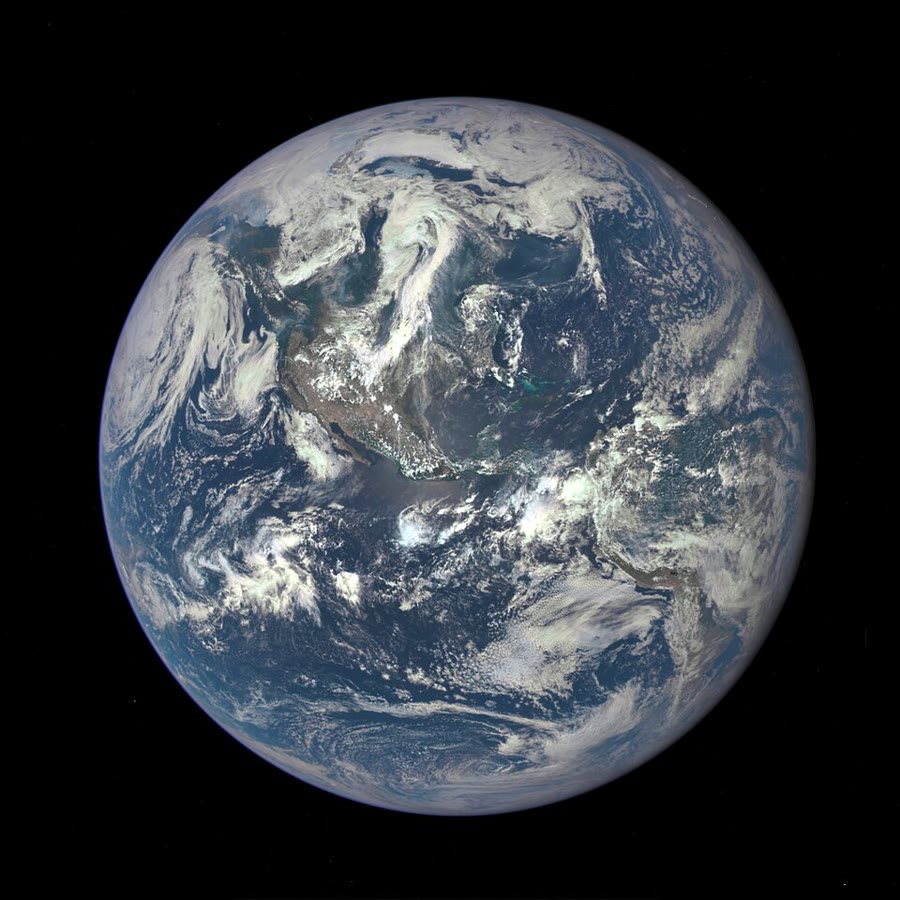
\includegraphics[width=0.55\linewidth]{images/book3/b1-epic-earth.jpg}

{\small The whole sunlit side of the Earth, photographed on 6 July 2015 by a
camera on the Deep Space Climate Observatory, a million miles away; North and
Central America are in the middle, with the turquoise shallow seas of the
Caribbean. Two weeks after the June solstice the Arctic, at the top, is lit all
round the clock. The bright clouds reflect much of the light that reaches them; the bluish tint is
sunlight scattered by the molecules of the air. (NASA Goddard Space Flight Center,
public domain, via Wikimedia Commons.)}
\label{fig:b1:radiation-heat-transport:epic}
\end{omfigure}
% ledger: commons:epic-earth (polar day: figdata/bachelor-1/insolation.py)

\begin{recall}
\Cref{ch:b1:spherical-astronomy} defined the \omterm{def:b1:spherical-astronomy:insolation}{insolation}, the power of sunlight
received per square metre of a horizontal surface at the top of the atmosphere,
$I = S_0(a/r)^2\sin h_\odot$ while the Sun is up, with $S_0 = \qty{1361}{W.m^{-2}}$
at the mean distance $a$; gave the Sun's \omterm{def:b1:spherical-astronomy:horizontal}{altitude} from its \omterm{def:b1:spherical-astronomy:equatorial}{hour angle} $H$, its
\omterm{def:b1:spherical-astronomy:equatorial}{declination} $\delta$ and the \omterm{def:b1:spherical-astronomy:geographic}{latitude} $\varphi$,
$\sin h_\odot = \sin\varphi\sin\delta + \cos\varphi\cos\delta\cos H$; and the \omterm{def:b1:spherical-astronomy:equatorial}{hour
angle} $H_0$ of sunset, $\cos H_0 = -\tan\varphi\tan\delta$
(\cref{prop:b1:spherical-astronomy:rising}). \Cref{ch:b1:comparative-planetology}
defined the \omterm{def:b1:comparative-planetology:albedo}{Bond albedo} of a planet and its \omterm{def:b1:comparative-planetology:equilibrium-temperature}{equilibrium temperature}. The physics
volumes give the inverse-square law for light, the radiation of a black body,
$\sigma T^4$ per square metre with $\sigma = \qty{5.670e-8}{W.m^{-2}.K^{-4}}$
(Stefan--Boltzmann), and the latent heat of a change of state. Book~2 showed that
the Earth intercepts on average a quarter of the solar constant, drew the global
energy budget of the Earth and checked that it balances, and described the
poleward transport of heat in words.
% ledger: earth:TSI, const:sigma, ipcc:budget-toa
\end{recall}

\section{Insolation with latitude and season}\label{sec:b1:radiation-heat-transport:insolation}

The instantaneous \omterm{def:b1:spherical-astronomy:insolation}{insolation} changes from minute to minute as the Sun crosses the
sky. For the climate, what counts is its sum over a day.

\begin{definition}[Daily-mean insolation]\label{def:b1:radiation-heat-transport:daily-insolation}
The \emph{daily-mean insolation}\index{daily-mean insolation} $\bar Q$ at a \omterm{def:b1:spherical-astronomy:geographic}{latitude}
on a given day is the instantaneous \omterm{def:b1:spherical-astronomy:insolation}{insolation} averaged over the 24 hours of that
day, nights included, the \omterm{def:b1:spherical-astronomy:equatorial}{declination} of the Sun and its distance being held at
their values for the day. It is a power per square metre of horizontal surface at
the top of the atmosphere, in \unit{W.m^{-2}}.
\end{definition}

Holding $\delta$ and $r$ fixed for a day is harmless: the \omterm{def:b1:spherical-astronomy:equatorial}{declination} changes by
at most \ang{0.4} a day, and the distance by less than \qty{0.03}{\percent}.
% ledger: earth:obliquity, earth:ecc (computed in figdata/bachelor-1/insolation.py)

\begin{theorem}[Daily-mean insolation]\label{thm:b1:radiation-heat-transport:daily}
At \omterm{def:b1:spherical-astronomy:geographic}{latitude} $\varphi$, on a day when the Sun's \omterm{def:b1:spherical-astronomy:equatorial}{declination} is $\delta$ and its
distance $r$,
\[
  \bar Q = \frac{S_0}{\pi}\left(\frac{a}{r}\right)^{2}
  \bigl(h_0\sin\varphi\sin\delta + \cos\varphi\cos\delta\sin h_0\bigr),
\]
where $h_0 \in [0, \pi]$ is the \omterm{def:b1:spherical-astronomy:equatorial}{hour angle} of sunset in radians: $\cos h_0 =
-\tan\varphi\tan\delta$ when $|\tan\varphi\tan\delta| \le 1$; $h_0 = \pi$ in the
polar day ($\tan\varphi\tan\delta > 1$); $h_0 = 0$, and $\bar Q = 0$, in the polar
night ($\tan\varphi\tan\delta < -1$).
\end{theorem}

\begin{proof}
The \omterm{def:b1:spherical-astronomy:equatorial}{hour angle} $H$ advances uniformly through $2\pi$ in a day, so the mean over
the day is the mean over $H \in [-\pi, \pi]$. The Sun is up for $-h_0 < H < h_0$,
where $\sin h_\odot > 0$, and the \omterm{def:b1:spherical-astronomy:insolation}{insolation} is zero otherwise. Hence
\[
  \bar Q = \frac{1}{2\pi}\int_{-h_0}^{h_0} S_0\left(\frac{a}{r}\right)^{2}
  \bigl(\sin\varphi\sin\delta + \cos\varphi\cos\delta\cos H\bigr)\,\mathrm dH ,
\]
which is $(S_0/2\pi)(a/r)^2\bigl(2h_0\sin\varphi\sin\delta +
2\cos\varphi\cos\delta\sin h_0\bigr)$.
The bounds come from \cref{prop:b1:spherical-astronomy:rising}: the \omterm{def:b1:spherical-astronomy:horizontal}{altitude} is
zero when $\cos H = -\tan\varphi\tan\delta$. If that number exceeds 1 in absolute
value, the Sun never crosses the horizon: when $\tan\varphi\tan\delta > 1$, the
integrand is positive for every $H$ and the integral runs over the whole day,
$h_0 = \pi$; when $\tan\varphi\tan\delta < -1$, it is negative for every $H$ and
the Sun never rises.
\end{proof}

Two special cases are worth knowing by heart. At the equator, $\varphi = 0$ and
$h_0 = \pi/2$ whatever the season:
\[
  \bar Q_\text{equator} = \frac{S_0}{\pi}\left(\frac{a}{r}\right)^{2}\cos\delta ,
\]
largest at the equinoxes, $S_0/\pi = \qty{433.2}{W.m^{-2}}$ at the mean distance.
At a pole in its summer, $h_0 = \pi$ and $\varphi = \pi/2$: $\bar Q_\text{pole} =
S_0(a/r)^2\sin\delta$, the Sun circling the sky at a constant \omterm{def:b1:spherical-astronomy:horizontal}{altitude} equal to
the \omterm{def:b1:spherical-astronomy:equatorial}{declination}.
% ledger: earth:TSI

\begin{proposition}[The polar summer]\label{prop:b1:radiation-heat-transport:polar-summer}
On a day of \omterm{def:b1:spherical-astronomy:equatorial}{declination} $\delta > 0$, the \omterm{def:b1:radiation-heat-transport:daily-insolation}{daily-mean insolation} at the North Pole
exceeds that at the equator if and only if $\pi\tan\delta > 1$, that is $\delta >
\ang{17.66}$. At the June solstice, $\delta = \ang{23.44}$, the ratio is $\pi\tan
\delta = 1.362$.
\end{proposition}

\begin{proof}
The two special cases above share the factor $(S_0/\pi)(a/r)^2$; their ratio is
$\pi\sin\delta/\cos\delta = \pi\tan\delta$, which exceeds 1 when $\tan\delta >
1/\pi$, $\delta > \arctan(1/\pi) = \ang{17.66}$. With the obliquity,
$\pi\tan\ang{23.44} = 1.362$.
\end{proof}
% ledger: earth:obliquity

With the Earth's orbit, the June solstice falls near aphelion, $(a/r)^2 = 0.968$:
the North Pole then receives \qty{524}{W.m^{-2}} as a daily mean, the equator
\qty{385}{W.m^{-2}}. Six months later the South Pole, near perihelion, receives
\qty{559}{W.m^{-2}}, \qty{6.7}{\percent} more than the North Pole had in its
summer: the ratio is exactly that of the two values of $(a/r)^2$. The figure below
shows $\bar Q$ over a whole year. The maxima are at the poles at the solstices;
the dark wedges are the polar nights, bounded by the \omterm{def:b1:spherical-astronomy:geographic}{latitude} $\ang{90} -
|\delta|$; the subsolar point, where the Sun passes overhead at noon, moves
between the tropics with the \omterm{def:b1:spherical-astronomy:equatorial}{declination}.
% ledger: earth:TSI, earth:ecc, earth:obliquity, nasa:earth-perihelion-longitude, usno:seasons-2026 (computed in figdata/bachelor-1/insolation.py)

\begin{omfigure}
\begin{tikzpicture}
\begin{axis}[omrecord, width=0.8\linewidth, height=6.4cm, view={0}{90},
  xmin=0, xmax=365, ymin=-90, ymax=90, xlabel={day of the year (from 1 January)},
  ylabel={latitude (\unit{\degree})}, xtick={0,60,...,360}, ytick={-90,-60,...,90},
  colormap/viridis, colorbar, point meta min=0, point meta max=560,
  colorbar style={ylabel={$\bar Q$ (\unit{W.m^{-2}})}, ytick={0,100,...,500}, width=0.3cm},
  axis on top, grid=none]
% figdata/bachelor-1/insolation.py; ledger: earth:TSI, earth:ecc, earth:obliquity, nasa:earth-perihelion-longitude, usno:tropical-year, usno:seasons-2026
\addplot3[surf, shader=interp, mesh/ordering=y varies, mesh/rows=73]
  table[x=day, y=lat, z=Q] {figdata/out/bachelor-1-insolation-grid.dat};
\addplot3[white, dashed, line width=0.8pt] table[x=day, y=decl, z expr=600] {figdata/out/bachelor-1-insolation-sun.dat};
\addplot3[white, line width=0.6pt, unbounded coords=jump] table[x=day, y=night_n, z expr=600] {figdata/out/bachelor-1-insolation-sun.dat};
\addplot3[white, line width=0.6pt, unbounded coords=jump] table[x=day, y=night_s, z expr=600] {figdata/out/bachelor-1-insolation-sun.dat};
\node[font=\scriptsize, text=white] at (axis cs:28,81,700) {polar night};
\node[font=\scriptsize, text=white] at (axis cs:172,-81,700) {polar night};
\node[font=\scriptsize, text=white, anchor=south] at (axis cs:172,26,700) {subsolar latitude};
\end{axis}
\end{tikzpicture}

{\small \omterm{def:b1:radiation-heat-transport:daily-insolation}{Daily-mean insolation} at the top of the atmosphere against the day of the
year and the \omterm{def:b1:spherical-astronomy:geographic}{latitude}, from \cref{thm:b1:radiation-heat-transport:daily} with
$S_0 = \qty{1361}{W.m^{-2}}$ and the Earth's orbit. Dashed: the subsolar \omterm{def:b1:spherical-astronomy:geographic}{latitude},
equal to the \omterm{def:b1:spherical-astronomy:equatorial}{declination}; solid: the edges of the polar nights. The summer poles
receive more than any other place on the Earth; the southern summer, near
perihelion, is the brighter of the two.}
\label{fig:b1:radiation-heat-transport:matrix}
\end{omfigure}
% ledger: earth:TSI, earth:ecc, earth:obliquity, nasa:earth-perihelion-longitude, usno:seasons-2026

Averaging $\bar Q$ over the year gives the annual-mean \omterm{def:b1:spherical-astronomy:insolation}{insolation} of each \omterm{def:b1:spherical-astronomy:geographic}{latitude}
(figure below): \qty{415.6}{W.m^{-2}} at the equator, \qty{328.3}{W.m^{-2}} at
\ang{40}, \qty{172.4}{W.m^{-2}} at either pole. The polar summer is intense but the
polar winter is dark, and over a year the equator receives \num{2.41} times as much
as a pole. The curve is the same in both hemispheres, although the southern summer
is the brighter; \cref{exo:b1:radiation-heat-transport:10} shows why.
% ledger: earth:TSI, earth:ecc, earth:obliquity (computed in figdata/bachelor-1/insolation.py)

\begin{omfigure}
\begin{tikzpicture}
\begin{axis}[omrecord, width=0.8\linewidth, height=5.6cm, xmin=-90, xmax=90, ymin=0, ymax=600,
  xlabel={latitude (\unit{\degree})}, ylabel={$\bar Q$ (\unit{W.m^{-2}})},
  xtick={-90,-60,...,90}, ytick={0,100,...,600}]
% figdata/bachelor-1/insolation.py; ledger: earth:TSI, earth:ecc, earth:obliquity, nasa:earth-perihelion-longitude
\addplot[omThm, line width=0.8pt] table[x=lat, y=Q_jun] {figdata/out/bachelor-1-insolation-annual.dat};
\addplot[omDef, line width=0.8pt] table[x=lat, y=Q_dec] {figdata/out/bachelor-1-insolation-annual.dat};
\addplot[black, line width=1.1pt] table[x=lat, y=Q_ann] {figdata/out/bachelor-1-insolation-annual.dat};
\addplot[black!60, dashed, domain=-90:90] {340.30};
\node[font=\scriptsize, text=omThm, anchor=west] at (axis cs:50,540) {June solstice};
\node[font=\scriptsize, text=omDef, anchor=east] at (axis cs:-50,575) {December solstice};
\node[font=\scriptsize, anchor=north] at (axis cs:-72,160) {annual mean};
\node[font=\scriptsize, text=black!60, anchor=south west] at (axis cs:-88,342) {global mean};
\end{axis}
\end{tikzpicture}

{\small \omterm{def:b1:radiation-heat-transport:daily-insolation}{Daily-mean insolation} against \omterm{def:b1:spherical-astronomy:geographic}{latitude} at the two solstices, and its
annual mean (black). The annual mean exceeds the global mean, \qty{340.3}{W.m^{-2}}
(dashed), between \ang{37} S and \ang{37} N, on \qty{60}{\percent} of the Earth's
surface.}
\label{fig:b1:radiation-heat-transport:annual}
\end{omfigure}
% ledger: earth:TSI, earth:ecc, earth:obliquity (computed in figdata/bachelor-1/insolation.py)

\begin{proposition}[The global mean]\label{prop:b1:radiation-heat-transport:global}
At every instant, the \omterm{def:b1:spherical-astronomy:insolation}{insolation} averaged over the whole sphere is $\tfrac14
S_0(a/r)^2$. Averaged over the year as well, it is $S_0/(4\sqrt{1 - e^2})$, where
$e$ is the eccentricity of the orbit: \qty{340.30}{W.m^{-2}} for the Earth, within
\qty{0.02}{\percent} of $S_0/4 = \qty{340.25}{W.m^{-2}}$.
\end{proposition}

\begin{proof}
The Earth, of radius $R$, intercepts the sunlight crossing a disc of area $\pi
R^2$, a power $S_0(a/r)^2\pi R^2$, which falls on the day hemisphere; spread over
the whole surface $4\pi R^2$, it gives the first result. The time average of
$(a/r)^2$ over the orbit is $1/\sqrt{1-e^2}$
(\cref{exo:b1:radiation-heat-transport:11}).
\end{proof}
% ledger: earth:TSI, earth:ecc

\section{Absorbed and emitted radiation}\label{sec:b1:radiation-heat-transport:toa}

Of the sunlight a \omterm{def:b1:spherical-astronomy:geographic}{latitude} receives, it reflects a fraction straight back, from
clouds, snow, ice, desert and, to a lesser degree, sea; it absorbs the rest, in
the air and at the surface. It also loses energy by emitting infrared radiation
to space, day and night.

\begin{definition}[Outgoing longwave radiation]\label{def:b1:radiation-heat-transport:olr}
The \emph{outgoing longwave radiation}\index{outgoing longwave radiation} (OLR)
is the power of infrared radiation leaving the top of the atmosphere towards space,
per square metre. The \emph{emission temperature}\index{emission temperature}
$T_e$ is the temperature of a black body that would emit the same power:
$\sigma T_e^4 = \text{OLR}$.
\end{definition}

The OLR comes partly from the surface, through the air where it is transparent
to infrared, and partly from the air and the cloud tops higher up. The \omterm{def:b1:radiation-heat-transport:olr}{emission
temperature} is a property of
the radiation, not the temperature of a particular level: it is lower than that
of the ground beneath, because the emitting layers are colder.
% ledger: ipcc:budget-surface, ipcc:budget-toa

\begin{definition}[Net radiation; radiative surplus and deficit]\label{def:b1:radiation-heat-transport:net-radiation}
The \emph{net radiation}\index{net radiation} at the top of the atmosphere is
\[
  R = \underbrace{(1 - \alpha)\,\bar Q}_{\text{absorbed solar}} - \text{OLR},
\]
where $\alpha$ is the local albedo, the fraction of the incoming sunlight reflected
to space; all three quantities are annual means at one \omterm{def:b1:spherical-astronomy:geographic}{latitude}. A \omterm{def:b1:spherical-astronomy:geographic}{latitude} where
$R > 0$ has a \emph{radiative surplus}\index{radiative surplus}; one where $R < 0$
has a \emph{radiative deficit}\index{radiative deficit}.
\end{definition}

Over the whole Earth the \omterm{def:b1:radiation-heat-transport:net-radiation}{net radiation} must average almost zero, since the planet
neither heats nor cools by more than a few tenths of a watt per square metre: the
latest assessment puts the imbalance at \qty{0.7}{W.m^{-2}}, on an incoming
\qty{340}{W.m^{-2}} of which \qty{100}{W.m^{-2}} are reflected (a global albedo of
\num{0.294}) and \qty{239}{W.m^{-2}} leave as infrared.
% ledger: ipcc:budget-toa, earth:albedo

The zonal profiles of this chapter come from a reanalysis, that is, a weather
forecasting system run over the past decades, which assimilates the observations of
each day and outputs a complete, consistent state of the atmosphere. The
reanalysis used here, from 1948 on, gives monthly means on a grid of 94 \omterm{def:b1:spherical-astronomy:geographic}{latitudes}
and 192 \omterm{def:b1:spherical-astronomy:geographic}{longitudes}; this chapter uses its averages over 1991--2020. Its radiation
fluxes are model outputs, forecasts constrained by the observations. The figure
below shows their zonal means against $\sin\varphi$, so that equal widths on the
axis are equal areas on the sphere.
% ledger: psl:ncep-r1, kalnay96:reanalysis, data:b3-ncep

\begin{omfigure}
\begin{tikzpicture}
\begin{axis}[omrecord, width=0.8\linewidth, height=6cm, xmin=-1, xmax=1, ymin=0, ymax=320,
  xlabel={latitude (\unit{\degree}, axis in $\sin\varphi$)}, ylabel={flux (\unit{W.m^{-2}})},
  xtick={-0.866,-0.5,0,0.5,0.866}, xticklabels={60 S,30 S,0,30 N,60 N},
  ytick={0,50,...,300}]
% figdata/bachelor-1/energy_balance.py; ledger: data:b3-ncep, psl:ncep-r1
\addplot[name path=asr, omProp, line width=1pt] table[x expr={sin(\thisrow{lat})}, y=asr] {figdata/out/bachelor-1-energy_balance-toa.dat};
\addplot[name path=olr, omThm, line width=1pt] table[x expr={sin(\thisrow{lat})}, y=olr] {figdata/out/bachelor-1-energy_balance-toa.dat};
\addplot[omProp!25] fill between[of=asr and olr, split, every segment no 1/.style={omDef!18}, every segment no 2/.style={omProp!30}, every segment no 3/.style={omDef!18}];
\node[font=\scriptsize, text=omProp!80!black] at (axis cs:-0.55,300) {absorbed solar};
\node[font=\scriptsize, text=omThm] at (axis cs:-0.2,226) {OLR};
\node[font=\scriptsize] at (axis cs:0,262) {surplus};
\node[font=\scriptsize] at (axis cs:0.86,178) {deficit};
\node[font=\scriptsize] at (axis cs:-0.86,178) {deficit};
\end{axis}
\end{tikzpicture}

{\small Zonal and annual mean absorbed solar radiation (orange) and \omterm{def:b1:radiation-heat-transport:olr}{outgoing
longwave radiation} (red) at the top of the atmosphere, from the NCEP-NCAR
Reanalysis~1, means 1991--2020 (data provided by the NOAA PSL, Boulder, Colorado,
USA, from their website at https://psl.noaa.gov). Shaded: the \omterm{def:b1:radiation-heat-transport:net-radiation}{radiative surplus} of
the low \omterm{def:b1:spherical-astronomy:geographic}{latitudes} and the deficits of the high \omterm{def:b1:spherical-astronomy:geographic}{latitudes}.}
\label{fig:b1:radiation-heat-transport:toa}
\end{omfigure}
% ledger: data:b3-ncep, psl:ncep-r1, kalnay96:reanalysis

The two curves have very different shapes. The absorbed sunlight falls from
\qty{288}{W.m^{-2}} near the equator to \qty{76}{W.m^{-2}} at \ang{81} N, by a
factor of \num{3.8}: the \omterm{def:b1:spherical-astronomy:insolation}{insolation} drops, and the albedo rises from \num{0.31} to
\num{0.57}, with the low Sun, the snow and the sea ice. The OLR falls only from
\qty{245}{W.m^{-2}} to \qty{192}{W.m^{-2}}, by a factor of \num{1.27}; the
\omterm{def:b1:radiation-heat-transport:olr}{emission temperatures} are \qty{256}{K} and \qty{241}{K}. The OLR is even slightly
lower at the equator, \qty{245}{W.m^{-2}}, than near \ang{20}, \qty{269}{W.m^{-2}}:
the clouds of the equatorial rain belt rise high and their cold tops emit little,
while the clearer subtropical skies let more infrared escape. Wherever the absorbed sunlight exceeds the OLR, the \omterm{def:b1:spherical-astronomy:geographic}{latitude} has a
surplus.
% ledger: data:b3-ncep (values computed in figdata/bachelor-1/energy_balance.py)

\begin{example}[The reanalysis's global budget]\label{ex:b1:radiation-heat-transport:global}
Averaged over the globe, the reanalysis receives \qty{341.9}{W.m^{-2}}, reflects
\qty{117.0}{W.m^{-2}} (an albedo of \num{0.342}), absorbs \qty{224.8}{W.m^{-2}} and
emits \qty{237.7}{W.m^{-2}}: a \omterm{def:b1:radiation-heat-transport:net-radiation}{net radiation} of \qty{-12.9}{W.m^{-2}}. The OLR is
within \qty{1.3}{W.m^{-2}} of the assessed \qty{239}{W.m^{-2}}, but the reflection
is \qty{17}{W.m^{-2}} larger than the assessed \qty{100}{W.m^{-2}}. A real
imbalance of this size would cool the Earth by \qty{6.6}{PW}; it is an error of
the model, not a property of the Earth, and the transport below is computed after
removing the global mean.
% ledger: data:b3-ncep, ipcc:budget-toa (computed in figdata/bachelor-1/energy_balance.py)
\end{example}

\section{Meridional heat transport}\label{sec:b1:radiation-heat-transport:transport}

\begin{definition}[Meridional heat transport]\label{def:b1:radiation-heat-transport:mht}
The \emph{meridional heat transport}\index{meridional heat transport} $T(\varphi)$
across the parallel of \omterm{def:b1:spherical-astronomy:geographic}{latitude} $\varphi$ is the energy carried northwards across
that parallel per unit time, by the atmosphere and the ocean together, in the annual
mean. It is counted positive northwards and measured in petawatts
(\qty{1}{PW} = \qty{e15}{W}).
\end{definition}

\begin{proposition}[Transport from the net radiation]\label{prop:b1:radiation-heat-transport:mht}
If the energy stored in each \omterm{def:b1:spherical-astronomy:geographic}{latitude} band does not change from year to year, then
for an Earth of radius $a_\oplus$,
\[
  T(\varphi) = 2\pi a_\oplus^2\int_{-\pi/2}^{\varphi} R(\varphi')\cos\varphi'\,
  \mathrm d\varphi' = -2\pi a_\oplus^2\int_{\varphi}^{\pi/2} R(\varphi')\cos
  \varphi'\,\mathrm d\varphi' ,
\]
and $T$ is extreme at the \omterm{def:b1:spherical-astronomy:geographic}{latitudes} where $R$ changes sign.
\end{proposition}

\begin{proof}
Take the polar cap south of the parallel $\varphi$ as a control volume, from the
bottom of the ocean to the top of the atmosphere (figure below). Energy enters or
leaves it in only two ways: as radiation at the top, a net power
$\int R\,\mathrm dA$, and by the transport across its rim, $-T(\varphi)$ (a
northward transport leaves the southern cap). The band between $\varphi'$ and
$\varphi' + \mathrm d\varphi'$ has area $\mathrm dA = 2\pi a_\oplus\cos\varphi'
\cdot a_\oplus\,\mathrm d\varphi'$. With no change of storage, the sum is zero:
$\int_{-\pi/2}^{\varphi} R\,2\pi a_\oplus^2\cos\varphi'\,\mathrm d\varphi' -
T(\varphi) = 0$. Applied to the whole Earth ($\varphi = \pi/2$, no rim), the same
balance gives $\int R\,\mathrm dA = 0$ over the sphere, whence the second form.
Differentiating, $T'(\varphi) = 2\pi a_\oplus^2 R(\varphi)\cos\varphi$, which
vanishes where $R$ changes sign.
\end{proof}
% ledger: earth:Rmean

\begin{omfigure}
\begin{tikzpicture}[>={Stealth[length=2mm]}, font=\scriptsize]
  \def\R{2.0}
  \def\ph{40}
  \fill[omDef!12] ({-\R*cos(\ph)},{\R*sin(\ph)}) arc[start angle=180-\ph, end angle=\ph, radius=\R]
     -- ({\R*cos(\ph)},{\R*sin(\ph)}) arc[start angle=0, end angle=-180, x radius={\R*cos(\ph)}, y radius={0.25*\R*cos(\ph)}] -- cycle;
  \draw[thick] (0,0) circle (\R);
  \draw[black!40] (-\R,0) arc[start angle=180, end angle=360, x radius=\R, y radius={0.25*\R}];
  \draw[black!40, dashed] (\R,0) arc[start angle=0, end angle=180, x radius=\R, y radius={0.25*\R}];
  \draw[omDef, thick] ({-\R*cos(\ph)},{\R*sin(\ph)}) arc[start angle=180, end angle=360, x radius={\R*cos(\ph)}, y radius={0.25*\R*cos(\ph)}];
  \draw[omDef, thick, dashed] ({\R*cos(\ph)},{\R*sin(\ph)}) arc[start angle=0, end angle=180, x radius={\R*cos(\ph)}, y radius={0.25*\R*cos(\ph)}];
  \node[anchor=west, black!60] at (\R+0.05,0) {equator};
  \node[anchor=west, omDef] at ({\R*cos(\ph)+0.1},{\R*sin(\ph)}) {parallel $\varphi$};
  \foreach \x in {-0.55,0.55} \draw[->, very thick, omProp] (\x,{\R*sin(\ph)-0.75}) -- (\x,{\R*sin(\ph)-0.1});
  \node[omProp!80!black, anchor=east] at ({-\R-0.1},{\R*sin(\ph)-0.4}) {$T(\varphi)$ crosses the rim};
  \foreach \a in {65,90,115} {
    \draw[->, omThm, decorate, decoration={snake, amplitude=0.6mm, segment length=2mm, post length=1.5mm}]
      ({(\R+0.05)*cos(\a)},{(\R+0.05)*sin(\a)}) -- ({(\R+0.75)*cos(\a)},{(\R+0.75)*sin(\a)});
  }
  \node[omThm, anchor=south] at (0,\R+0.8) {net radiation $R < 0$ over the cap};
\end{tikzpicture}

{\small The control volume of \cref{prop:b1:radiation-heat-transport:mht}, drawn
for the cap north of the parallel $\varphi$ (shaded): in a steady state, what the
cap loses by radiation at the top of the atmosphere (red) is what the atmosphere
and the ocean bring in across its rim (orange).}
\label{fig:b1:radiation-heat-transport:cap}
\end{omfigure}

Applied to the reanalysis, with its global mean of \qty{-12.9}{W.m^{-2}} subtracted
from $R$ at every \omterm{def:b1:spherical-astronomy:geographic}{latitude}, the proposition gives the curve below. The transport is
northward in the northern hemisphere and southward in the southern one, always
towards the pole. It peaks at \qty{4.1}{PW} near \ang{38} N and \qty{4.5}{PW} near
\ang{32} S, where $R$ minus its mean changes sign; across \ang{40} N it is
\qty{4.11}{PW}. It is small at the equator, where the surplus of each hemisphere
is exported to its own pole.
% ledger: data:b3-ncep (computed in figdata/bachelor-1/energy_balance.py)

\begin{omfigure}
\begin{tikzpicture}
\begin{axis}[omrecord, width=0.8\linewidth, height=6cm, xmin=-90, xmax=90, ymin=-5.5, ymax=6.4,
  xlabel={latitude (\unit{\degree})}, ylabel={northward transport (\unit{PW})},
  xtick={-90,-60,...,90}, ytick={-4,-2,...,4}]
% figdata/bachelor-1/energy_balance.py; ledger: data:b3-ncep, trenberth:transport
\addplot[black!40, domain=-90:90] {0};
\addplot[black, line width=1.1pt] table[x=lat, y=T_PW] {figdata/out/bachelor-1-energy_balance-transport.dat};
\addplot[omMeth, dashed, line width=0.9pt] table[x=lat, y=T_PW] {figdata/out/bachelor-1-energy_balance-latent.dat};
\addplot[only marks, mark=square*, mark size=2pt, omThm] coordinates {(43,5.0)};
\node[font=\scriptsize, anchor=east] at (axis cs:28,4.4) {total};
\node[font=\scriptsize, text=omMeth, anchor=north] at (axis cs:42,0.9) {latent heat};
\node[font=\scriptsize, text=omThm, anchor=south] at (axis cs:43,5.2) {atmosphere alone (Trenberth and Caron)};
\end{axis}
\end{tikzpicture}

{\small The \omterm{def:b1:radiation-heat-transport:mht}{meridional heat transport} implied by the reanalysis's \omterm{def:b1:radiation-heat-transport:net-radiation}{net radiation}
(black) and its latent-heat part (dashed green, from the evaporation and the
precipitation, \cref{sec:b1:radiation-heat-transport:latent}); NCEP-NCAR
Reanalysis~1, means 1991--2020, data provided by the NOAA PSL. Square: the peak of
the atmospheric transport alone in an estimate constrained by satellite
measurements of the radiation, \qty{5.0}{PW} at \ang{43} N (Trenberth and Caron,
2001).}
\label{fig:b1:radiation-heat-transport:transport}
\end{omfigure}
% ledger: data:b3-ncep, psl:ncep-r1, trenberth:transport

The square on the figure is a warning. A study of the years 1985--1989, when a
satellite experiment measured the radiation at the top of the atmosphere reliably,
computed the transport of the atmosphere from the winds, temperatures and moisture
of two reanalyses: the atmosphere alone carries \qty{5.0}{PW} at \ang{43} N, more
than this reanalysis's \qty{4.0}{PW} for the atmosphere and the ocean together. The
same study found that the model-generated fluxes of the reanalysis agree less well
with independent ocean estimates than fluxes derived from the observations. Once
the global mean is removed, the transport depends only on how $R$ varies with
\omterm{def:b1:spherical-astronomy:geographic}{latitude}, and this reanalysis's \omterm{def:b1:radiation-heat-transport:net-radiation}{net radiation} varies too little from the tropics to
the poles. The shape of the curve, its peaks in the \omterm{def:b1:spherical-astronomy:geographic}{mid-latitudes} and its
near-symmetry, can be trusted; its height falls at least a fifth short.
% ledger: trenberth:transport, tc01:method, data:b3-ncep (computed in figdata/bachelor-1/energy_balance.py)

Who carries the heat? The same study finds that the ocean carries
more than the atmosphere only between the equator and \ang{17} N; at \ang{35},
where the total transport peaks in each hemisphere, the atmosphere carries
\qty{78}{\percent} of it in the north and \qty{92}{\percent} in the south. The
ocean's share is the subject of \cref{ch:b1:ocean-circulation}, the atmosphere's
of \cref{ch:b1:atmospheric-circulation}.
% ledger: trenberth:transport

\begin{method}[Transport from zonal bands]\label{met:b1:radiation-heat-transport:bands}
\begin{enumerate}
  \item Divide the cap poleward of the \omterm{def:b1:spherical-astronomy:geographic}{latitude} of interest into bands; for each,
        take the mean \omterm{def:b1:spherical-astronomy:insolation}{insolation} $\bar Q_i$, albedo $\alpha_i$ and OLR$_i$.
  \item Compute the \omterm{def:b1:radiation-heat-transport:net-radiation}{net radiation} of each band, $R_i = (1 - \alpha_i)\bar Q_i -
        \text{OLR}_i$, and subtract the global mean of $R$ if it is not zero.
  \item Compute the area of each band, $A_i = 2\pi a_\oplus^2(\sin\varphi_{i,2} -
        \sin\varphi_{i,1})$, with $a_\oplus = \qty{6371}{km}$.
  \item The transport across the rim is minus the net power of the cap,
        $-\sum_i R_i A_i$, positive towards the pole; divide by \num{e15} for
        petawatts.
\end{enumerate}
\end{method}
% ledger: earth:Rmean

\section{Latent and sensible heat}\label{sec:b1:radiation-heat-transport:latent}

The surface of the Earth absorbs most of the sunlight, but the atmosphere radiates
most of the infrared to space. The surface hands energy to the air in three ways:
by its own infrared radiation, by warming the air in contact with it, and by
evaporating water, whose latent heat is released wherever the vapour condenses.
That place may be thousands of kilometres away: the latent heat travels with the
wind.

\begin{definition}[Latent and sensible heat fluxes; Bowen ratio]\label{def:b1:radiation-heat-transport:surface-fluxes}
The \emph{latent heat flux}\index{latent heat flux} $LE$ is the power per square
metre that the surface loses by evaporation: the evaporation rate $E$, in
\unit{kg.m^{-2}.s^{-1}}, times the latent heat of vaporisation $L$. The
\emph{sensible heat flux}\index{sensible heat flux} $H$ is the power per square
metre that the surface passes to the air by conduction and turbulence, warming
it. Both are counted positive upwards. Their ratio $B = H/LE$ is the
\emph{Bowen ratio}\index{Bowen ratio}.
\end{definition}

Near \qty{15}{\celsius}, $L = \qty{2.4655}{MJ.kg^{-1}}$. The \omterm{def:b1:radiation-heat-transport:surface-fluxes}{Bowen ratio} is small
over the sea and over wet ground, where water is plentiful, and large over dry land.
In the reanalysis it is \num{0.09} at the equator, \num{0.37} at \ang{25} N, the
\omterm{def:b1:spherical-astronomy:geographic}{latitude} of the great hot deserts, and negative at \ang{70} N, where the snow and
ice surfaces are colder than the air above them in the annual mean, so that the
sensible \omterm{def:b1:heat-budget:heat-flow}{heat flows} downwards. Averaged over the globe, the reanalysis gives $LE =
\qty{82.5}{W.m^{-2}}$ and $H = \qty{15.2}{W.m^{-2}}$, a \omterm{def:b1:radiation-heat-transport:surface-fluxes}{Bowen ratio} of \num{0.18};
the assessed values are \qty{82}{W.m^{-2}} and \qty{21}{W.m^{-2}}, a ratio of
\num{0.26}.
% ledger: nist:water-latent, data:b3-ncep, ipcc:budget-surface (computed in figdata/bachelor-1/energy_balance.py)

Book~2 turned the \omterm{def:b1:radiation-heat-transport:surface-fluxes}{latent heat flux} into a depth of water evaporated each year. The
converse turns a rainfall, which a gauge can collect, into an energy flux.

\begin{proposition}[Precipitation as an energy flux]\label{prop:b1:radiation-heat-transport:rain}
A precipitation rate of \qty{1}{m} of water per year releases in the atmosphere,
where its vapour condensed, a mean power of
\[
  \frac{\qty{1000}{kg.m^{-2}} \times \qty{2.4655e6}{J.kg^{-1}}}{\qty{3.156e7}{s}}
  = \qty{78.1}{W.m^{-2}} .
\]
\end{proposition}

\begin{proof}
A layer of water \qty{1}{m} deep has a mass of \qty{1000}{kg} per square metre.
Condensing the vapour that forms it releases $1000L$; a year of \num{365.25} days
lasts \qty{3.156e7}{s}.
\end{proof}
% ledger: nist:water-latent

\begin{example}[The water cycle as an energy flux]\label{ex:b1:radiation-heat-transport:rain}
The global water cycle brings \num{373000} cubic kilometres of rain and snow to the
ocean every year and \num{113000} to the land: spread over the Earth's
\qty{5.10e8}{km^2}, \qty{0.953}{m} per year, which releases
\qty{74}{W.m^{-2}} by \cref{prop:b1:radiation-heat-transport:rain}. The reanalysis
rains \qty{2.82}{mm} a day, \qty{1.03}{m} a year, \qty{80}{W.m^{-2}}. Both are close
to the assessed \omterm{def:b1:radiation-heat-transport:surface-fluxes}{latent heat flux} of \qty{82}{W.m^{-2}}, whose uncertainty range is
\qtyrange{72}{85}{W.m^{-2}}: over the years, the water that evaporates comes down
again, and the latent heat taken from the surface is all given to the air.
% ledger: trenberth:water-cycle, earth:Rmean, data:b3-ncep, ipcc:budget-surface (computed in calc/ch27.py)
\end{example}

The balance holds for the globe, not for each \omterm{def:b1:spherical-astronomy:geographic}{latitude}, and the difference is a
transport (figure below). In the subtropics the sea evaporates more water than
falls there: $LE$ exceeds $LP$, the latent heat of the precipitation. The
equatorial rain belt and the \omterm{def:b1:spherical-astronomy:geographic}{mid-latitudes} receive more rain than they
evaporate. Between the two, the vapour is carried by the wind, and with it
latent heat. By the argument of \cref{prop:b1:radiation-heat-transport:mht},
applied to the integral of $LE - LP$, the reanalysis carries
\qty{1.4}{PW} of latent heat northwards across \ang{40} N, a third of its total
transport there; the latent transport is drawn dashed on the transport figure above.
% ledger: data:b3-ncep (computed in figdata/bachelor-1/energy_balance.py)

\begin{omfigure}
\begin{tikzpicture}
\begin{axis}[omrecord, width=0.8\linewidth, height=6cm, xmin=-1, xmax=1, ymin=-60, ymax=200,
  xlabel={latitude (\unit{\degree}, axis in $\sin\varphi$)}, ylabel={flux (\unit{W.m^{-2}})},
  xtick={-0.866,-0.5,0,0.5,0.866}, xticklabels={60 S,30 S,0,30 N,60 N},
  ytick={-50,0,50,...,200}]
% figdata/bachelor-1/energy_balance.py; ledger: data:b3-ncep, nist:water-latent
\addplot[black!40, domain=-1:1] {0};
\addplot[omMeth, line width=1pt] table[x expr={sin(\thisrow{lat})}, y=lh] {figdata/out/bachelor-1-energy_balance-surface.dat};
\addplot[omDef, line width=1pt] table[x expr={sin(\thisrow{lat})}, y=lp] {figdata/out/bachelor-1-energy_balance-surface.dat};
\addplot[omThm, dashed, line width=0.9pt] table[x expr={sin(\thisrow{lat})}, y=sh] {figdata/out/bachelor-1-energy_balance-surface.dat};
\node[font=\scriptsize, text=omMeth, anchor=south] at (axis cs:-0.35,118) {$LE$};
\node[font=\scriptsize, text=omDef, anchor=south] at (axis cs:0.06,168) {$LP$};
\node[font=\scriptsize, text=omThm, anchor=south] at (axis cs:0.2,24) {$H$};
\end{axis}
\end{tikzpicture}

{\small Zonal and annual means of the \omterm{def:b1:radiation-heat-transport:surface-fluxes}{latent heat flux} $LE$ (green), of the latent
heat released by the precipitation, $LP$ (blue), and of the \omterm{def:b1:radiation-heat-transport:surface-fluxes}{sensible heat flux}
$H$ (red, dashed), from the NCEP-NCAR Reanalysis~1, means 1991--2020 (data provided
by the NOAA PSL). Where $LE > LP$, in the subtropics, water vapour is exported;
where $LP > LE$, under the rain belts, it is imported.}
\label{fig:b1:radiation-heat-transport:surface}
\end{omfigure}
% ledger: data:b3-ncep, psl:ncep-r1, nist:water-latent

\section{The surface energy budget}\label{sec:b1:radiation-heat-transport:surface}

The global budget drawn in Book~2 can be read as one equation for the surface.

\begin{proposition}[Surface energy balance]\label{prop:b1:radiation-heat-transport:surface}
Let $R_n$ be the \omterm{def:b1:radiation-heat-transport:net-radiation}{net radiation} at the surface, absorbed sunlight plus infrared
received from the air minus infrared emitted, and $G$ the power per square metre
that goes into the ground or the ocean below. Then, per square metre,
\[
  R_n = LE + H + G .
\]
In the global mean, $R_n = 160 + 342 - 398 = \qty{104}{W.m^{-2}}$, of which
\qty{82}{W.m^{-2}} go into evaporation, \qty{21}{W.m^{-2}} into the \omterm{def:b1:radiation-heat-transport:surface-fluxes}{sensible heat
flux}, and $G \approx \qty{1}{W.m^{-2}}$, within the rounding of the figures, into
the ocean and the ground.
\end{proposition}

\begin{proof}
Take as a system a thin layer at the surface, with no heat capacity of its own.
Energy reaches it only as radiation ($R_n$, net) and leaves it only as the latent
and \omterm{def:b1:radiation-heat-transport:surface-fluxes}{sensible heat fluxes} upwards and the conduction or mixing downwards; the
balance is the equation. The numbers are the assessed global means.
\end{proof}
% ledger: ipcc:budget-surface

\begin{omfigure}
\begin{tikzpicture}[font=\scriptsize, >={Stealth[length=2.2mm, width=2mm]}, line width=1.3pt]
  \fill[omExo!35] (0,0) rectangle (9.6,0.6);
  \fill[omDef!10] (0,0.6) rectangle (9.6,4.2);
  \draw[thin, black!60] (0,0.6) -- (9.6,0.6);
  \node[anchor=west, black!70] at (0.1,0.3) {ground and ocean};
  \node[anchor=west, black!70] at (0.1,3.9) {atmosphere};
  \draw[->, omProp!90!black] (1.6,3.4) -- (1.6,0.65);
  \node[anchor=east, align=right] at (1.5,2.2) {160\\absorbed\\solar};
  \draw[->, omThm!50] (2.6,3.4) -- (2.6,0.65);
  \node[anchor=west, align=left] at (2.7,2.2) {342\\infrared\\from the air};
  \draw[->, omThm!80!black] (4.8,0.65) -- (4.8,3.4);
  \node[anchor=west, align=left] at (4.9,2.2) {398\\emitted};
  \draw[->, omMeth!80!black] (6.9,0.65) -- (6.9,3.4);
  \node[anchor=west, align=left] at (7.0,2.6) {82 $LE$};
  \draw[->, omMeth!80!black] (8.2,0.65) -- (8.2,2.0);
  \node[anchor=west, align=left] at (8.3,1.6) {21 $H$};
  \draw[->, black!70] (5.9,0.55) -- (5.9,-0.35);
  \node[anchor=west] at (6.0,-0.15) {$G \approx 1$};
  \draw[thin, black!50, decorate, decoration={brace, amplitude=4pt}] (1.0,4.35) -- (5.2,4.35)
     node[midway, above=3pt, black] {$R_n = 160 + 342 - 398 = 104$};
  \draw[thin, black!50, decorate, decoration={brace, amplitude=4pt}] (6.6,4.35) -- (9.3,4.35)
     node[midway, above=3pt, black] {$LE + H + G = 104$};
\end{tikzpicture}

{\small The global mean surface energy balance in \unit{W.m^{-2}}, from the
values of the IPCC Sixth Assessment Report, Working Group~I, Figure~7.2. The \omterm{def:b1:radiation-heat-transport:net-radiation}{net
radiation} absorbed by the surface, \qty{104}{W.m^{-2}}, is handed to the
atmosphere mostly as latent heat; $G$, the small remainder, warms the ocean.}
\label{fig:b1:radiation-heat-transport:budget}
\end{omfigure}
% ledger: ipcc:budget-surface, ipcc:heating

The \omterm{def:b1:radiation-heat-transport:surface-fluxes}{latent heat flux}, four fifths of $R_n$, is the larger of the two non-radiative
terms by far: over the globe, the surface cools mainly by evaporating water. The
small $G$ is the climate system's heating, the \qty{0.7}{W.m^{-2}} of the
budget at the top of the atmosphere; nine tenths of it is stored in the
ocean.
% ledger: ipcc:budget-surface, ipcc:budget-toa, ipcc:heating

\begin{remark}[Local and global]\label{rem:b1:radiation-heat-transport:local}
At a single place, $G$ is far from small: it is large and positive by day and in
summer, negative by night and in winter, and it averages out only over a day or a
year. Over the ocean, the heat stored in the \omterm{def:b1:fluid-envelopes-structure:ocean-layers}{mixed layer} can also be carried away
sideways by the currents: the local balance must then include the ocean's
transport, as the balance of a \omterm{def:b1:spherical-astronomy:geographic}{latitude} band includes the atmosphere's.
\end{remark}

\section{Exercises}

\begin{exercise}[$\star$]\label{exo:b1:radiation-heat-transport:1}
(a)~Compute $S_0/\pi$ with $S_0 = \qty{1361}{W.m^{-2}}$. (b)~On the day of the March
equinox, the \omterm{def:b1:radiation-heat-transport:daily-insolation}{daily-mean insolation} at the equator is \qty{436.7}{W.m^{-2}}. Deduce
$(a/r)^2$ and $r/a$ on that day. (c)~At the June solstice, $(a/r)^2 = 0.9683$ and
$\delta = \ang{23.44}$. Compute the \omterm{def:b1:radiation-heat-transport:daily-insolation}{daily-mean insolation} at the equator.
% ledger: earth:TSI, earth:obliquity (computed in figdata/bachelor-1/insolation.py)
\end{exercise}

\begin{exercise}[$\star$]\label{exo:b1:radiation-heat-transport:2}
The annual-mean \omterm{def:b1:spherical-astronomy:insolation}{insolation} is \qty{415.6}{W.m^{-2}} at the equator and
\qty{172.4}{W.m^{-2}} at the poles; the global mean is \qty{340.3}{W.m^{-2}}.
(a)~By what factor does the equator exceed the poles? (b)~The annual mean equals the
global mean at \ang{37.0} N and S. What fraction of the Earth's surface lies between
these two parallels? (c)~Why does this make the annual-mean curve look more
favourable to the high \omterm{def:b1:spherical-astronomy:geographic}{latitudes} than the Earth's surface really is?
% ledger: earth:TSI, earth:ecc, earth:obliquity (computed in figdata/bachelor-1/insolation.py)
\end{exercise}

\begin{exercise}[$\star$]\label{exo:b1:radiation-heat-transport:3}
In the reanalysis the OLR is \qty{244.9}{W.m^{-2}} near the equator,
\qty{192.3}{W.m^{-2}} at \ang{81} N and \qty{237.7}{W.m^{-2}} in the global mean.
(a)~Compute the three \omterm{def:b1:radiation-heat-transport:olr}{emission temperatures}. (b)~Over the same \omterm{def:b1:spherical-astronomy:geographic}{latitudes}, the
absorbed sunlight falls from \qty{287.7}{W.m^{-2}} to \qty{75.8}{W.m^{-2}}. Compare
the two ratios. (c)~What does the comparison imply for the \omterm{def:b1:radiation-heat-transport:net-radiation}{net radiation}?
% ledger: data:b3-ncep, const:sigma
\end{exercise}

\begin{exercise}[$\star$]\label{exo:b1:radiation-heat-transport:4}
The reanalysis's global mean precipitation is \qty{2.82}{mm} a day. (a)~Convert it to
metres per year. (b)~Compute the latent heat it releases, in \unit{W.m^{-2}}, with
\cref{prop:b1:radiation-heat-transport:rain}. (c)~Compare with the reanalysis's own
global \omterm{def:b1:radiation-heat-transport:surface-fluxes}{latent heat flux}, \qty{82.5}{W.m^{-2}}, and explain why the two should agree
over many years.
% ledger: data:b3-ncep, nist:water-latent
\end{exercise}

\begin{exercise}[$\star\star$]\label{exo:b1:radiation-heat-transport:5}
(a)~At the June solstice ($\delta = \ang{23.44}$, $(a/r)^2 = 0.9683$), compute the
\omterm{def:b1:radiation-heat-transport:daily-insolation}{daily-mean insolation} at the North Pole. (b)~At the December solstice, $(a/r)^2 =
1.0334$; compute it at the South Pole and the ratio of the two. (c)~The Sun stands
only \ang{23.4} above the horizon at the pole: explain how the pole can still beat
the equator.
% ledger: earth:TSI, earth:obliquity, earth:ecc (computed in figdata/bachelor-1/insolation.py)
\end{exercise}

\begin{exercise}[$\star\star$]\label{exo:b1:radiation-heat-transport:6}
At \ang{40} N, compute the \omterm{def:b1:spherical-astronomy:equatorial}{hour angle} of sunset, the length of the day and the
\omterm{def:b1:radiation-heat-transport:daily-insolation}{daily-mean insolation} (a)~at the June solstice, with $(a/r)^2 = 0.9683$, $\delta =
\ang{23.44}$; (b)~at the December solstice, with $(a/r)^2 = 1.0334$, $\delta =
\ang{-23.44}$. (c)~What share of the ratio between the two comes from the distance
to the Sun?
% ledger: earth:TSI, earth:obliquity (computed in figdata/bachelor-1/insolation.py)
\end{exercise}

\begin{exercise}[$\star\star$]\label{exo:b1:radiation-heat-transport:7}
The reanalysis gives the following zonal means (\unit{W.m^{-2}}):
\begin{center}
\small
\begin{tabular}{|l|cccc|}
\hline
\omterm{def:b1:spherical-astronomy:geographic}{latitude} & \ang{0} & \ang{25} N & \ang{45} N & \ang{70} N \\
$LE$ & 96.0 & 96.4 & 52.4 & 23.7 \\
$H$ & 8.9 & 36.1 & 17.7 & $-3.6$ \\
\hline
\end{tabular}
\end{center}
(a)~Compute the \omterm{def:b1:radiation-heat-transport:surface-fluxes}{Bowen ratio} at each \omterm{def:b1:spherical-astronomy:geographic}{latitude}. (b)~Which \omterm{def:b1:spherical-astronomy:geographic}{latitude} has the largest
ratio? What kind of surface explains it? (c)~Interpret the sign of $H$ at
\ang{70} N.
% ledger: data:b3-ncep
\end{exercise}

\begin{exercise}[$\star\star$]\label{exo:b1:radiation-heat-transport:8}
The assessed global budget at the top of the atmosphere is \qty{340}{W.m^{-2}}
incoming, \qty{100}{W.m^{-2}} reflected, \qty{239}{W.m^{-2}} emitted; the reanalysis
gives \qty{341.9}{}, \qty{117.0}{} and \qty{237.7}{W.m^{-2}}. (a)~Compute the two
albedos and the two \omterm{def:b1:radiation-heat-transport:net-radiation}{net radiations}. (b)~Which term explains most of the
reanalysis's imbalance? (c)~Show that if the global mean of $R$ were not removed,
\cref{prop:b1:radiation-heat-transport:mht} would leave a transport of
\qty{-6.6}{PW} at the North Pole, and explain why that is impossible.
% ledger: ipcc:budget-toa, data:b3-ncep, earth:Rmean
\end{exercise}

\begin{exercise}[$\star\star$]\label{exo:b1:radiation-heat-transport:9}
In the reanalysis, the belt between \ang{30} S and \ang{30} N has a mean \omterm{def:b1:radiation-heat-transport:net-radiation}{net
radiation}, after removal of the global mean, of \qty{+33}{W.m^{-2}}. (a)~Compute the
area of the belt and its total surplus in petawatts. (b)~If the two hemispheres
exported the surplus equally, how much would cross each of the parallels \ang{30}
N and \ang{30} S? (c)~The reanalysis gives \qty{4.00}{PW} northwards across \ang{30}
N and \qty{4.50}{PW} southwards across \ang{30} S. What does the difference say?
% ledger: data:b3-ncep, earth:Rmean (computed in calc/ch27.py)
\end{exercise}

\begin{exercise}[$\star\star\star$]\label{exo:b1:radiation-heat-transport:10}
The \omterm{def:b1:radiation-heat-transport:daily-insolation}{daily-mean insolation} depends on the \omterm{def:b1:spherical-astronomy:geographic}{latitude}, the \omterm{def:b1:spherical-astronomy:equatorial}{declination} and the factor
$(a/r)^2$. (a)~With Kepler's second law, $r^2\,\mathrm d\lambda/\mathrm dt = h$
constant, where $\lambda$ is the Sun's \omterm{def:b1:spherical-astronomy:ecliptic}{ecliptic} \omterm{def:b1:spherical-astronomy:geographic}{longitude}, show that the energy a
\omterm{def:b1:spherical-astronomy:geographic}{latitude} receives while $\lambda$ advances by $\mathrm d\lambda$ does not depend on
$r$. (b)~Deduce that the annual-mean \omterm{def:b1:spherical-astronomy:insolation}{insolation} at \omterm{def:b1:spherical-astronomy:geographic}{latitude} $\varphi$ equals that at
$-\varphi$, although the southern summer is brighter. (c)~In the orbit model of this
chapter, the Sun takes \num{186.4} days from the March to the September equinox and
\num{178.8} days back. Explain how these numbers fit (b).
% ledger: earth:ecc, earth:obliquity, nasa:earth-perihelion-longitude, usno:tropical-year (computed in calc/ch27.py)
\end{exercise}

\begin{exercise}[$\star\star\star$]\label{exo:b1:radiation-heat-transport:11}
(a)~Using Kepler's second law in the form $r^2\,\mathrm d\lambda/\mathrm dt = h$
and the area of the ellipse, $\pi a b = hP/2$ over a period $P$, show that the time
average of $(a/r)^2$ over an orbit is $a/b = 1/\sqrt{1 - e^2}$. (b)~Complete the
proof of \cref{prop:b1:radiation-heat-transport:global}. (c)~With $e = 0.0167$,
compute the global annual mean and its difference from $S_0/4$.
% ledger: earth:TSI, earth:ecc
\end{exercise}

\begin{exercise}[$\star\star\star$]\label{exo:b1:radiation-heat-transport:12}
The reanalysis gives a total transport of \qty{4.10}{PW} across \ang{35} N and
\qty{4.02}{PW} across \ang{43} N. (a)~Using the partition of Trenberth and Caron at
\ang{35} N (atmosphere \qty{78}{\percent}), split the reanalysis's total into an
atmospheric and an oceanic part. (b)~The same study finds \qty{5.0}{PW} for
the atmosphere alone at \ang{43} N. What does this say about the reanalysis?
(c)~Removing the global mean of $R$ does not cure this error. Why not?
% ledger: trenberth:transport, data:b3-ncep
\end{exercise}

\section{Problem: How much heat crosses the 40th parallel?}

\begin{problem}[{Weekend problem --- the energy budget of the cap north of
\ang{40} N}]
\label{pb:b1:radiation-heat-transport:1}
% values: calc/ch27.py; the band data are the NCEP-NCAR Reanalysis 1 means 1991-2020
% (data:b3-ncep), averaged over 10-degree bands in figdata/bachelor-1/energy_balance.py
The cap of the Earth north of \ang{40} N, which holds most of Europe, Russia
and Canada, radiates more energy to space than it absorbs from
the Sun. This problem measures the deficit, and so the heat that the atmosphere and
the ocean bring across the 40th parallel. Use $S_0 = \qty{1361}{W.m^{-2}}$,
$a_\oplus = \qty{6371}{km}$, $\sigma = \qty{5.670e-8}{W.m^{-2}.K^{-4}}$, $L =
\qty{2.4655e6}{J.kg^{-1}}$. The band data are the reanalysis's means for 1991--2020.

\medskip
\noindent\textbf{Part I --- Sunlight north of \ang{40} N.} On the June solstice
$\delta = \ang{23.44}$ and $(a/r)^2 = 0.9683$; on the December solstice $\delta =
\ang{-23.44}$ and $(a/r)^2 = 1.0334$; on the March equinox $\delta = 0$ and
$(a/r)^2 = 1.0081$.
\begin{enumerate}
  \item Compute the \omterm{def:b1:radiation-heat-transport:daily-insolation}{daily-mean insolation} at \ang{40} N on the three days.
  \item Compute it at \ang{80} N on the same three days.
  \item In June, \ang{80} N receives more than \ang{40} N. Explain why, with the
        \omterm{def:b1:spherical-astronomy:equatorial}{hour angles} of sunset.
  \item By integrating the theorem over the year, one finds annual means of
        \qty{306.9}{}, \qty{260.3}{}, \qty{213.7}{}, \qty{185.6}{} and
        \qty{173.8}{W.m^{-2}} at \ang{45}, \ang{55}, \ang{65}, \ang{75} and
        \ang{85} N. Compare with the band \omterm{def:b1:spherical-astronomy:insolation}{insolation} of the table in Part~II and
        give two reasons for the differences.
  \item The reanalysis's global mean \omterm{def:b1:spherical-astronomy:insolation}{insolation} is \qty{341.9}{W.m^{-2}}. What
        value of $S_0$ does it imply?
  \item Compute the area of the cap north of \ang{40} N and the fraction of the
        Earth's surface it covers.
\end{enumerate}

\medskip
\noindent\textbf{Part II --- Absorbed and emitted.} The reanalysis gives, for five
bands of the cap:
\begin{center}
\small
\begin{tabular}{|l|ccccc|}
\hline
band & \ang{40}--\ang{50} & \ang{50}--\ang{60} & \ang{60}--\ang{70} & \ang{70}--\ang{80} & \ang{80}--\ang{90} \\
$\bar Q$ (\unit{W.m^{-2}}) & 308.4 & 262.4 & 217.3 & 188.7 & 176.1 \\
albedo $\alpha$ & 0.358 & 0.393 & 0.426 & 0.510 & 0.576 \\
OLR (\unit{W.m^{-2}}) & 226.1 & 210.3 & 201.3 & 197.4 & 191.6 \\
\hline
\end{tabular}
\end{center}
\begin{enumerate}[resume]
  \item Compute the absorbed solar radiation of each band.
  \item Compute the \omterm{def:b1:radiation-heat-transport:net-radiation}{net radiation} of each band. Which band has the largest
        deficit?
  \item Compute the \omterm{def:b1:radiation-heat-transport:olr}{emission temperature} of each band.
  \item From \ang{40}--\ang{50} to \ang{80}--\ang{90}, by what factor does the
        absorbed sunlight fall, and by what factor the OLR?
  \item Give two reasons why the albedo increases towards the pole.
  \item Why does the OLR vary so much less than the absorbed sunlight?
\end{enumerate}

\medskip
\noindent\textbf{Part III --- The net radiation of the cap.}
\begin{enumerate}[resume]
  \item Compute the area of each band and check that they add up to the area of
        Question~6.
  \item Compute the net radiative power of each band and of the whole cap, in
        petawatts.
  \item Compute the mean albedo of the cap, weighting each band by its incoming
        sunlight, and compare it with the reanalysis's global albedo of \num{0.342}.
  \item The reanalysis's global mean \omterm{def:b1:radiation-heat-transport:net-radiation}{net radiation} is \qty{-12.90}{W.m^{-2}}. What
        would this mean if it were real? Compare with the assessed imbalance of
        \qty{+0.7}{W.m^{-2}}.
  \item Subtract this global mean from the \omterm{def:b1:radiation-heat-transport:net-radiation}{net radiation} of each band and compute
        again the net power of the cap.
  \item Explain, with \cref{prop:b1:radiation-heat-transport:mht}, why the
        corrected deficit of the cap must be brought in across the 40th parallel.
\end{enumerate}

\medskip
\noindent\textbf{Part IV --- The transport and its latent share.} Over the cap the
reanalysis gives a mean \omterm{def:b1:radiation-heat-transport:surface-fluxes}{latent heat flux} of \qty{42.4}{W.m^{-2}} and a mean
precipitation of \qty{1.95}{mm} a day; over the globe, the mean of $LE - LP$ is
\qty{2.07}{W.m^{-2}}.
\begin{enumerate}[resume]
  \item Compute the transport across \ang{40} N, in petawatts.
  \item Compute the latent heat $LP$ released by the cap's precipitation, in
        \unit{W.m^{-2}}, and compare it with $LE$.
  \item Removing the global mean of $LE - LP$, compute the latent heat brought into
        the cap as water vapour, in petawatts.
  \item What fraction of the transport across \ang{40} N is latent heat?
  \item Taking the share of the atmosphere found by Trenberth and Caron at \ang{35} N,
        \qty{78}{\percent}, as valid at \ang{40} N, split the transport into
        latent heat, the rest of the atmospheric transport, and the ocean.
  \item The same study finds \qty{5.0}{PW} for the atmosphere alone at
        \ang{43} N. Is your answer an upper or a lower bound of the truth?
  \item How much heat crosses the 40th parallel north, in petawatts?
\end{enumerate}
\end{problem}
